%Interfaces
This section provides a detailed description of all inputs into and outputs from the UPRM system. It also gives a description of the hardware, software and communication interfaces and provides basic prototypes of the user interface.

\subsubsection{User Interfaces}
	The first time the user loads the UPRM system on their browser, they should be greeted with a login screen. If the user is registered then they should be able to input their username and password and be able to enter the UPRM system. Before being given complete access to the UPRM system after successful username/password authentication, the user will be asked to give a UPRM system generated OTP that will be dynamically created and communicated with the user on some third-party service such as email or SMS.
	
	\textbf{Mockup of a login and OTP interface for the UPRM system: }\\
	\centerline{\fbox{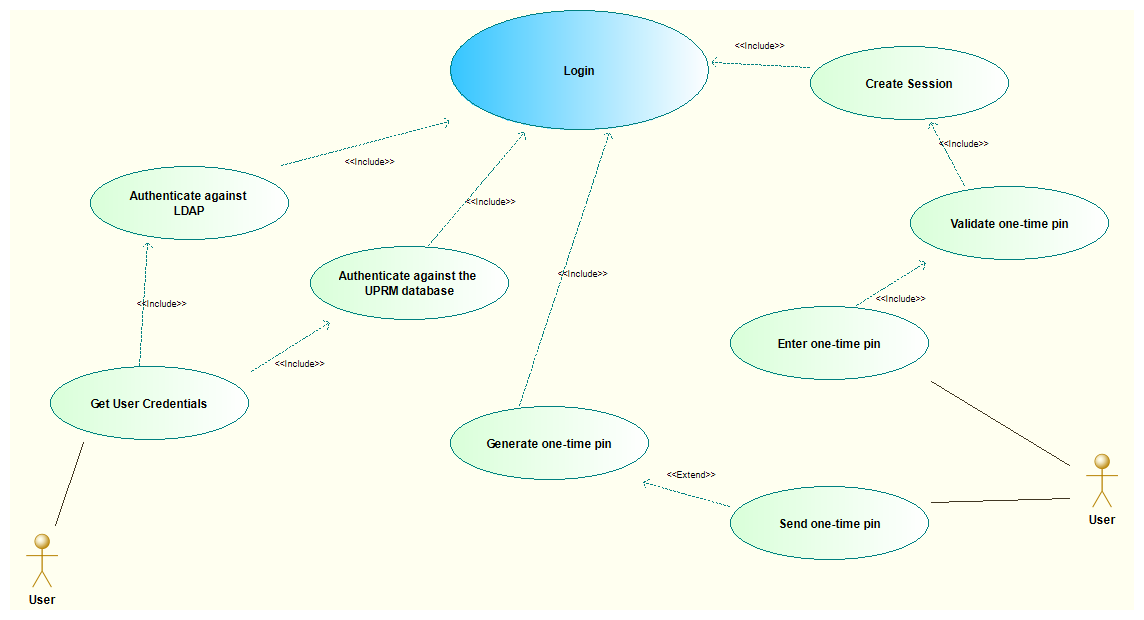
\includegraphics[scale=0.4]{Interfaces/Login.png}}}\\
	\centerline{\fbox{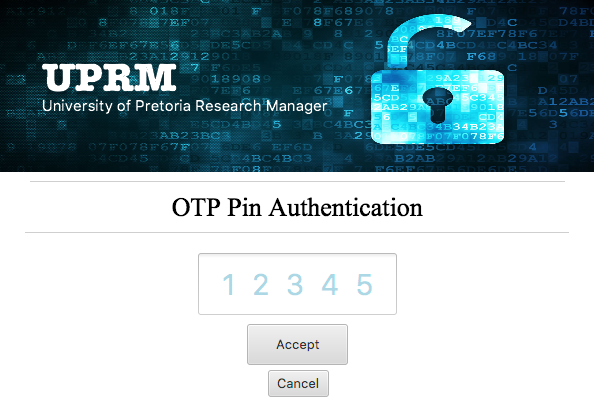
\includegraphics[scale=0.4]{Interfaces/otp.png}}}
	
	As soon as the user has entered the correct OTP, then the user will have access to the UPRM system. Once inside the UPRM system they can navigate to any functionality that is available on their user permission level. On the RMSQ the user will be asked to refine a query for their search on statistics of the projects. Some details they could be asked for are as follow:
	\begin{itemize}
		\item Name of a project.
		\item The dates of projects.
		\item The status type of a project.
		\item The specific venue for a project.
		\item A specific author for a project.
	\end{itemize}
	As soon as the user has entered their desired query information, the user will have to be able to choose between displaying the statistics gathered or exporting the report by making use of the RMR functionality.\\
	\textbf{Mockup of a RMSQ interface for the UPRM system: }\\
	\centerline{\fbox{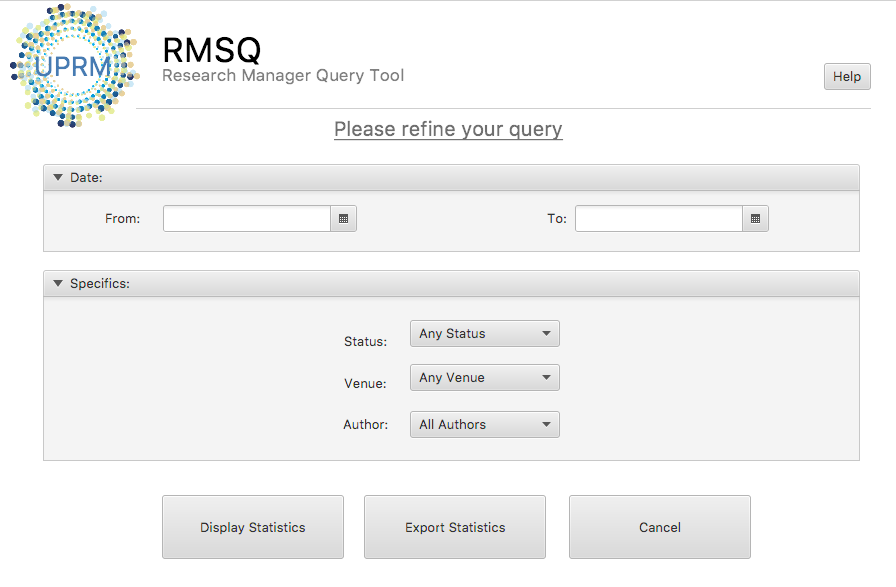
\includegraphics[scale=0.4]{Interfaces/rmsq.png}}}\\
	
	The RMVC interface will require the user to enter the following information:
	\begin{itemize}
		\item Name of the venue.
		\item Name of the organisation responsible for the venue.
		\item The date for the deadline of submissions, or marking a checkbox to indicate that no deadline exists.
		\item Contact details to which submissions will be sent.
	\end{itemize}
	
	\textbf{Mockup of a RMVC interface for the UPRM system: }\\
	\centerline{\fbox{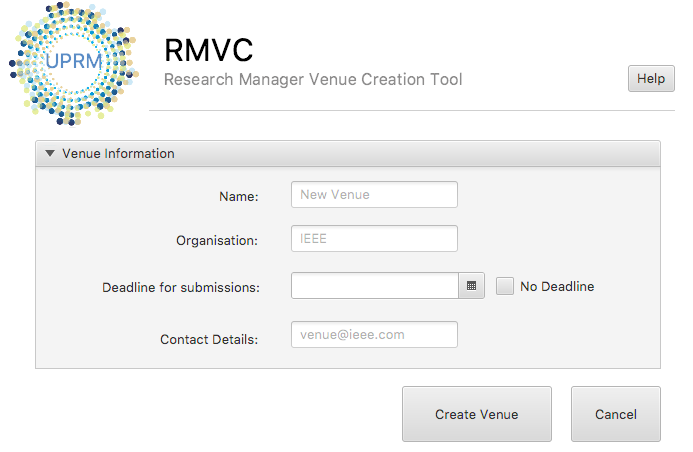
\includegraphics[scale=0.4]{Interfaces/rmvc.png}}}\\
	
	
\subsubsection{Hardware Interfaces}
	As UPRM will only be interfaced through a web portal, UPRM does not have any direct hardware interfaces. UPRM will have a responsive design and will hence work on any physical hardware platform that has an internet connection and a web browser.
	
\subsubsection{Software Interfaces}
	Most of UPRM communication will be with the database system. The communication with the database will consist of reading, writing and modifying data based on the permission levels set by the administrator for that user. The UPRM consist of mainly three software interfaces namely:
	\begin{itemize}
		\item A web server.
		\item A database server.
		\item A client interface.
	\end{itemize}

\subsubsection{Communication Interfaces}
	The communication between the different parts of the system is important since they depend on each
	other. However, in what way the communication is achieved is not important for the system and is
	therefore handled by the underlying operating systems.
